% Jason R. Blevins - Curriculum Vitae
%
% Copyright (C) 2004-2014 Jason R. Blevins <jrblevin@sdf.org>
% http://jblevins.org/
%
% You may use use this document as a template to create your own CV
% and you may redistribute the source code freely.  No attribution is
% required in any resulting documents.  I do ask that you please leave
% this notice and the above URL in the source code if you choose to
% redistribute this file.

\documentclass[11pt,letterpaper]{article}

\usepackage{hyperref}
\hypersetup{colorlinks,linkcolor={blue},citecolor={blue}}
\usepackage{geometry}
% Underline vertical space
\usepackage{soul}
        \setul{0ex}{}

% Fonts
\usepackage[T1]{fontenc}
\usepackage{times}
%\usepackage[urw-garamond]{mathdesign}
\usepackage{graphicx}
\usepackage{natbib}
\usepackage{bibentry}
\bibliographystyle{plainnat}

% Set your name here
\def\name{Leimin Tian}

% The following metadata will show up in the PDF properties
\hypersetup{
  colorlinks = true,
  urlcolor = blue,
  pdfauthor = {Leimin Tian},
  pdfkeywords = {Leimin Tian, 2021},
  pdftitle = {Leimin Tian - CV},
  pdfsubject = {CV - Leimin Tian - 2021},
  pdfpagemode = UseNone
}

\geometry{
  body={6.5in, 9.0in},
  left=1.0in,
  top=1.0in
}

% Customize page headers
\pagestyle{myheadings}
\markright{\name}
\thispagestyle{empty}

% Custom section fonts
\usepackage{sectsty}
\sectionfont{\rmfamily\mdseries\Large}
\subsectionfont{\rmfamily\mdseries\itshape\large}

% Other possible font commands include:
% \ttfamily for teletype,
% \sffamily for sans serif,
% \bfseries for bold,
% \scshape for small caps,
% \normalsize, \large, \Large, \LARGE sizes.

% Don't indent paragraphs.
\setlength\parindent{0em}

% Make lists without bullets and compact spacing
%\renewenvironment{itemize}{
%  \begin{list}{}{
%    \setlength{\leftmargin}{1.5em}
%    \setlength{\itemsep}{0.25em}
%    \setlength{\parskip}{0pt}
%    \setlength{\parsep}{0.25em}
%  }
%}{
%  \end{list}
%}

\begin{document}
%\url{https://www.tudelft.nl/over-tu-delft/werken-bij-tu-delft/vacatures/details/?jobId=745}
%To apply, please e-mail:
%\begin{itemize}
%\item a detailed CV with a short letter of motivation,
%\item a personal research and teaching statement (max 3 pages),
%\item contact information of three scientific referees,
%\item a publication list,
%\item an abstract of your PhD thesis,
%\item links to two selected publications
%\end{itemize}
%Please send all your application information combined into one single pdf file named 'TUD00368_YourLastName.pdf' to vacancies-EEMCS@tudelft.nl
\nobibliography{MyPaperList}

\begin{minipage}[b]{0.55\textwidth}
  {\huge Dr. Leimin Tian \\}
  \\
  {\large Research Fellow \\}
  \\
  \href{https://www.monash.edu/engineering/robotics}{Robotics}, ECSE, Engineering \\
  \href{https://www.monash.edu/it/hcc/human-centred-ai-lab}{Human-Centred AI Lab} \\
  \href{https://www.monash.edu/data-futures-institute}{Data Futures Institute} \\
  Monash University \\
  \\
  Melbourne, Australia \\
  Phone: (+61) (0) 432 987 082 \\
  Email: \href{mailto:Leimin.Tian@monash.edu}{Leimin.Tian@monash.edu} \\
  Website: \href{https://tianleimin.github.io/}{\ul{https://tianleimin.github.io/}}\\
  ORCID: \href{https://orcid.org/0000-0001-8559-5610}{0000-0001-8559-5610}
\end{minipage}
\hfill
\begin{minipage}[b]{0.4\textwidth}
  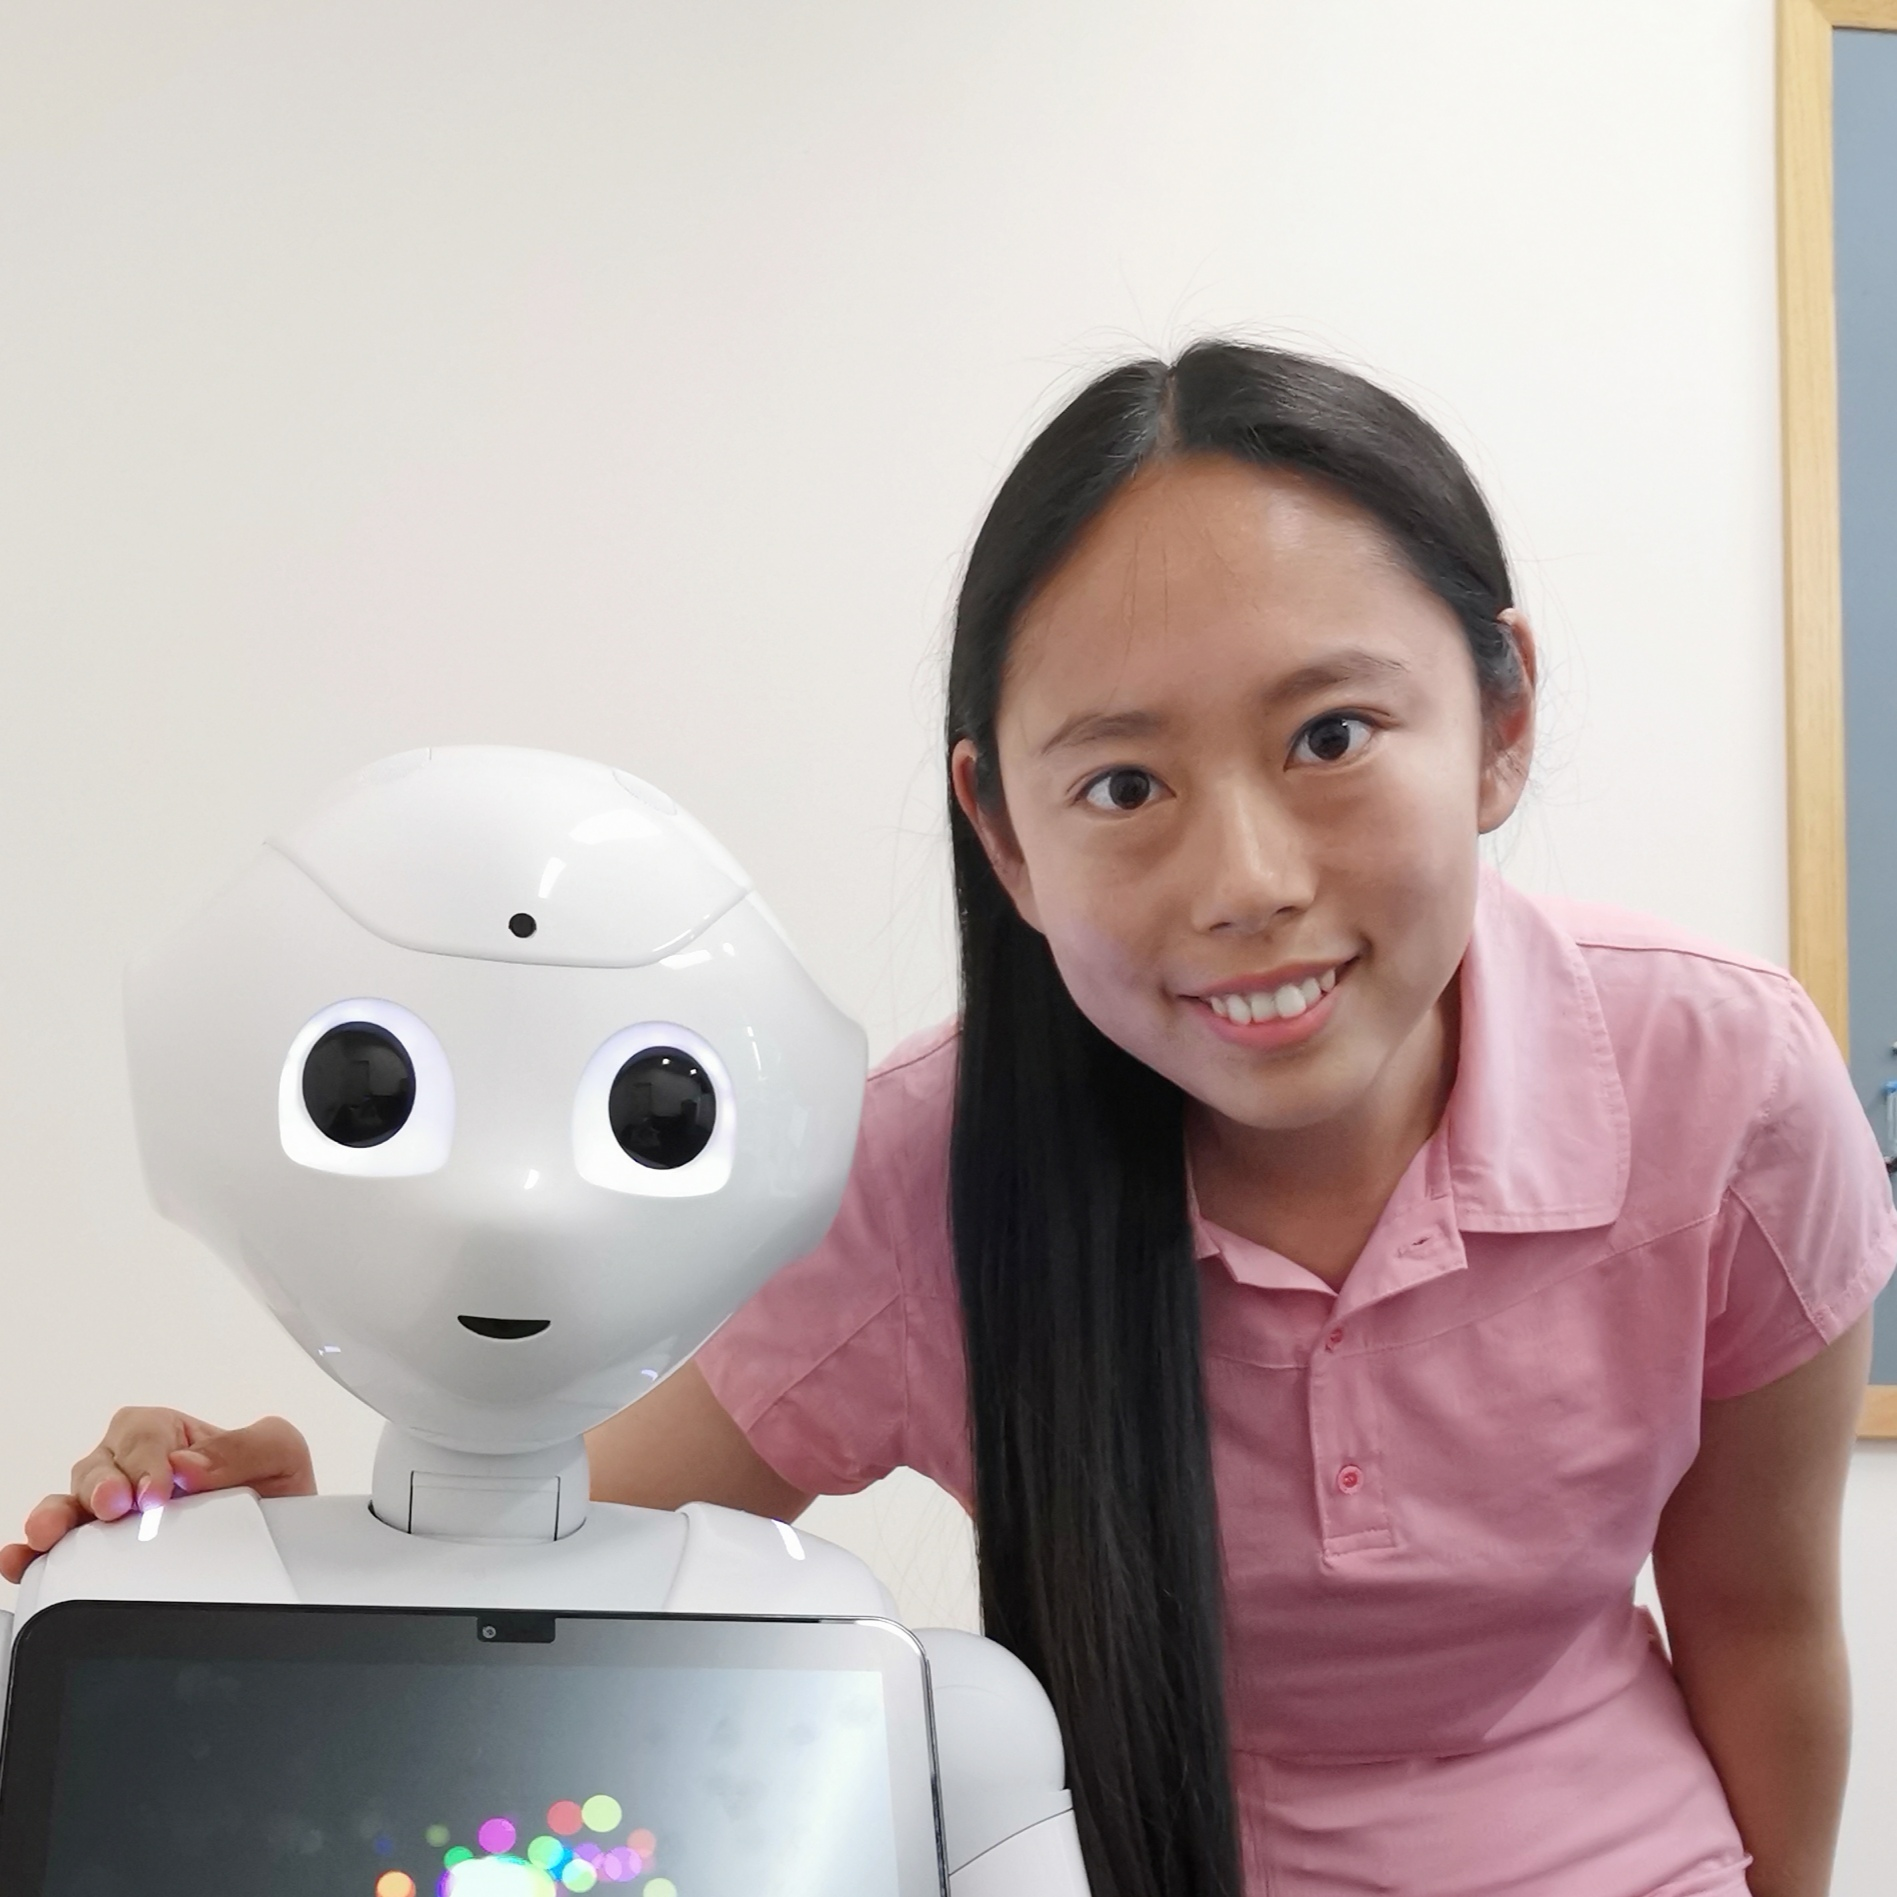
\includegraphics[width=\textwidth]{me}
\end{minipage}

\bigskip

\subsection*{Research Interests}
Affective Computing, Human-Robot Interaction, Human-Centred AI, Multimodal Behavioural Analytics, Social Robotics, Dialogue Systems, Digital Health, Speech Processing, Natural Language Processing

\subsection*{Education}
\begin{itemize}
  \item Ph.D. in Informatics. The University of Edinburgh. 2013--2018.
  \begin{itemize}
    \item \emph{Thesis:} ``Recognizing Emotions in Spoken Dialogue with Acoustic and Lexical Cues''
    \item \emph{Supervisors:} Prof. Johanna D. Moore and Dr. Catherine Lai
  \end{itemize}
  \item M.Sc. in Artificial Intelligence (\emph{with Distinction}). The University of Edinburgh. 2012--2013.
  \begin{itemize}
    \item \emph{Dissertation:} ``Emotion Recognition using Feature-Level Fused Audio-Visual Data''
    \item \emph{Supervisors:} Prof. Johanna D. Moore and Dr. Catherine Lai
  \end{itemize}
  \item B.Eng. in Artificial Intelligence. Beijing University of Posts and Telecommunications. 2008--2012.
  \begin{itemize}
    \item \emph{Dissertation:} ``An Application of Audio-Visual Emotion Recognition''
    \item \emph{Supervisors:} Prof. Xiaojie Wang and Dr. Yongbin Liu
  \end{itemize}
\end{itemize}

\subsection*{Grants and Awards}
\begin{itemize}
  \item Best Reviewer Awards (top 5\% of reviewers) at ICMI 2021
  \item Monash University Interdisciplinary Research Seed Grant. Aug.~2021--Aug.2022. 
  \begin{itemize}
    \item \emph{Project:} ``Transforming measurement of how unsafe someone feels when bike riding''
    \item \emph{Investigators:} Dr. Ben Beck (project lead), Prof. Dana Kuli{\'c}, Dr. Akansel Cosgun, Dr. Leimin Tian, and Dr. Joanne Caldwell Odgers
    \item \emph{Grant:} AUD 50,000, application success rate 16\%
  \end{itemize}
  \item Monash University Interdisciplinary Research Seed Grant. Jan.~2020--Dec.2021. 
  \begin{itemize}
    \item \emph{Project:} ``\href{https://www.monash.edu/research/better-governance-and-policy/projects-and-research/robots-in-public-space}{Understanding Robots in Public Spaces}: Interdisciplinary Insights for Public Policy''
    \item \emph{Investigators:} Prof. Shanti Sumartojo (project lead), Prof. Dana Kuli{\'c}, Dr. Leimin Tian, and Prof. Michael Mintrom
    \item \emph{Grant:} AUD 50,000, application success rate 16\%
  \end{itemize}
  \item Monash University Faculty of IT Early Career Researcher Seed Grant. July~2019--Aug.2020.
  \begin{itemize}
    \item \emph{Project:} ``Developing a Robot Teleoperation Framework for Simulation Studies''
    \item \emph{Investigator:} Dr. Leimin Tian
    \item \emph{Grant:} AUD 13,000
  \end{itemize}
  \item Fiorella De Rosis Award for the best Doctoral Consortium paper at the sixth International Conference on Affective Computing and Intelligent Interaction (ACII 2015).
  \item Full PhD scholarship funded by the University of Edinburgh.
\end{itemize}

\subsection*{Work Experiences}
\begin{itemize}
  \item \emph{Research Fellow.} Monash University. 23rd~July~2018--Present.
  \item \emph{Consultant.} EmoTech Ltd. 19th~Sep.~2016--19th~Dec.~2016.
  \begin{itemize}
    \item \emph{AI of Emotion Project:} Designed and developed the emotion recognition, emotional interaction modelling, and emotion synthesis modules of Olly, a domestic personal assistant robot. 
  \end{itemize}
  \item \emph{Research Intern.} Chinese Academy of Science, Institute of Psychology. Jul.~2011--Aug.~2011.
  \begin{itemize}
    \item \emph{Projects:} 
      \begin{itemize}
      \item Facial Expression Recognition System %\\Wrote Matlab code for extracting Gabor features
      \item Affect Modelling with Galvanic Skin Responses (GSR) %\\Collected GSR data for emotion recognition
      \item Creativity Test for Chinese University students %\\Performed Williams Creative Tendency Scale analysis
      \end{itemize}
    \item \emph{Supervisor:} Prof. Xiaolan Fu
  \end{itemize}
  \item \emph{Research Assistant.} Beijing University of Posts and Telecommunications, Department of Computer Science. Jun.~2010--Nov.~2011.
  \begin{itemize}
    \item \emph{Project:} Intelligent Tutoring System for Pre-School Children
    \item \emph{Supervisor:} Prof. Xiaojie Wang
  \end{itemize}
\end{itemize}


\subsection*{Teaching and Supervision}
\begin{itemize}
  \item \emph{Co-instructor} of course ECE4078 (Intelligent Robotics): Monash University. Aug--Nov 2020 / 021.
  \item \emph{Co-supervisor} of PhD candidate Subra Muthusamy: ``Multimodal Anlaysis of Patients with Epileptic Seizure and Psychogenic Non-Epileptic Seizure''. Monash Health. Feb 2020--Present.
  \item \emph{Co-supervisor} of PhD candidate Chathurika Palliya Guruge: ``Designing Multimodal Interfaces for Early Diagnosis of Dementia''. Monash University. Feb 2019--Feb 2020.
  \item \emph{Primary or co-supervisor} of Master thesis, Honor's thesis, and final year projects: Monash University. 2019--Present.
  \begin{itemize}
    \item Liam Whittle: ``Incorporating Social Norms and context in Reinforcement Learning'' (Master thesis)
    \item Faezeh Fazel: ``Explainable AI for Visual Snow Syndrome'' (Master thesis)
	\item Shuyi Cao (completed): ``Modelling Human-Human Emotion Dynamics in Spoken Dialogue System'' (Master thesis)
    \item Shujie Zhou (completed): ``Exploring the Role of Emotions in Human-Multi-Agent Collaboration'' (Master thesis)
    \item Duc Huy Tran (completed): ``Modelling Human-Human Emotion Dynamics in Spoken Dialogue'' (Honor's thesis)
  \end{itemize}
  \item \emph{Co-supervisor} of MSc dissertations: The University of Edinburgh. 2016--2017.
  \begin{itemize}
    \item Stanley Wang: ``Representation Learning for Emotion Recognition''
    \item Chenyu Wang: ``Automatic Detection of Non-Verbal Vocalisations in Spoken Dialogues''
    \item Xinran Shi: ``Automatic Detection of Disfluencies in Spoken Dialogues''
  \end{itemize}
\end{itemize}


\subsection*{Technical Skills}
\begin{itemize}
  \item \emph{Programming languages:} Python (primary)
  \item \emph{Robotic platforms:} Pepper, NAO, Cozmo, Fetch
  \item \emph{Machine learning and deep learning:} Keras, PyTorch, TensorFlow, Scikit-Learn, R, WEKA, SPSS
  \item \emph{Cloud platforms:} Amazon Web Services, Google Colab, Google ASR, Google Dialogflow
  \item \emph{Signal processing and annotation:} OpenFace, OpenPose, OpenSMILE, Praat, ELAN, Amazon Mechanical Turk
  \item \emph{Other:} ROS, Linux, \LaTeX
\end{itemize}

\subsection*{Services}
\begin{itemize}
  \item \emph{Regular reviewer}: ACII, ICMI, ICSR, IROS, RO-MAN, IEEE Transactions on Affective Computing.
  \item \emph{Publicity chair}: ACII 2019, ICMI 2020.
  \item \emph{Associate editor} and \href{https://underline.io/events/28/sessions?eventSessionId=365}{\emph{Session chair}} at RO-MAN 2020.
  \item \emph{Organizer.} \href{http://kdd.cs.ksu.edu/Workshops/IJCAI-2020-AffComp/index.html}{IJCAI Workshop on Artificial Intelligence in Affective Computing}. 2019--Present.
  \item \emph{Junior Executive Committee Member.}  \href{https://aaac.cs.nott.ac.uk/}{Association for the Advancement of Affective Computing (AAAC)}. Feb.~2018--Present.
  \item \emph{Committee Member.} Faculty of IT's Early Career Academic committee. Feb.~2019--Feb.~2020.
  \item \emph{Organizer.} \href{https://sites.google.com/monash.edu/socialroboticsworkshop/home}{Social Robotics Workshop}. 12th~Aug.~2019.
  \item \emph{Committee Member.} British Science Association (Edinburgh Branch). Sep.~2012--Jun.~2018.
\end{itemize}

\subsection*{Public Engagement and Media Presence}
\begin{itemize}
  \item \href{https://www.mediapolisjournal.com/2020/08/robotic-logics-of-public-space/}{Robotics Logics of Public Space in the COVID Pandemic}. 13th~Aug.~2020, Mediapolis.
  \item \href{https://medium.com/shes-building-a-robot/leimin-tian-9843a1080cd8}{She's Building a Robot: an Interview with Mick Liubinskas}. 15th~July~2019.
  \item \href{https://www.eventbrite.co.uk/e/meet-ai-series-6-tickets-39512362540#}{Affective Computing: What We Do and Do Not Know}. 22nd~Nov.~2017, Emotech Ltd \& Cocoon Networks, London, UK.
  \item \href{https://youtu.be/6Cd_BquE95Q}{Girls in Tech}: in \href{https://youtu.be/dMMtaeqWGlg}{English} and in \href{https://youtu.be/G0cfdK36wTE}{Mandarin}. 8th~Mar.~2017
\end{itemize}

\subsection*{Scientific Referees}
Available upon request
% \begin{itemize}
% \item Prof. Dana Kuli{\'c}
%   \begin{itemize}
%   \item Current supervisor
%   \item Professor at Department of Electrical and Computer Systems Engineering and Department of Mechanical and Aerospace Engineering, Monash University, Australia
%   \item Email: \href{mailto:Dana.Kulic@monash.edu}{Dana.Kulic@monash.edu}
%   \end{itemize}
% \item \emph{Prof. Sharon Oviatt}
%   \begin{itemize}
%   \item Current supervisor
%   \item Professor at Engineering Office of the Dean, Monash University, Australia
%   \item Email: \href{mailto:Sharon.Oviatt@monash.edu}{Sharon.Oviatt@monash.edu}
%   \end{itemize}
% \item \emph{Prof. Johanna D. Moore}
%   \begin{itemize}
%   \item PhD supervisor
%   \item Professor at School of Informatics, the University of Edinburgh, UK
%   \item Email: \href{mailto:J.Moore@ed.ac.uk}{J.Moore@ed.ac.uk}
%   \end{itemize}
% \end{itemize}

\subsection*{Full Publication List}
Please see \href{https://scholar.google.com/citations?user=d-PQpWgAAAAJ&hl=en}{my Google Scholar} for an up-to-date list of publications.

~\\~
Top 5:
\begin{enumerate}
\item \bibentry{tian2021taxonomy}
\item \bibentry{tian2021redesigning}
\item \bibentry{zhou2020would}
\item \bibentry{tian2018polarity}
\item \bibentry{tian2017recognizinginduced}
\end{enumerate}

Other:
\begin{enumerate}
\item \bibentry{tian2021applied}
\item \bibentry{mintrom2021robots}
\item \bibentry{coronado2021towards}
\item \bibentry{sumartojo2021imagining}
\item \bibentry{cao2021causal}
\item \bibentry{mckenzie2021discrepancies}
\item \bibentry{muszynski2021workshop}
\item \bibentry{tian2020user}
\item \bibentry{lai2019detecting}
\item \bibentry{muszynski2019recognizing}
\item \bibentry{williams2018dnn}
\item \bibentry{tian2017recognizingemotions}
\item \bibentry{tian2016recognizing}
\item \bibentry{tian2015recognizingACII}
\item \bibentry{tian2015emotion}
\item \bibentry{tian2015recognizingLaugtherWorkshop}
\item \bibentry{moore2014word}
\end{enumerate}


%\newpage
%\bibliographystyle{plainnat}
%\bibliography{MyPaperList}

\end{document}